\documentclass[12pt,a4paper]{report}
\usepackage[utf8]{inputenc}
\usepackage{graphicx}
\usepackage{geometry}
\usepackage{listings}
\usepackage{xcolor}
\usepackage{hyperref}
\usepackage{booktabs}

\geometry{margin=1in}

\title{\textbf{Design and Develop a Tool for Digital Forensic of Images}}
\author{Shivshankar Mali \\ Roll No: 49, Division: C}
\date{Academic Year: 2026--27}

\begin{document}

\begin{titlepage}
    \centering
    {\large JSPM's Bhivarabai Sawant Institute of Technology and Research \\ Wagholi, Pune -- 412207\par}
    \vspace{0.5cm}
    {\large Department of Computer Engineering\par}
    \vspace{1.5cm}
    
\includegraphics[width=4cm]{logo.png}\par
    \vspace{1cm}
    {\LARGE \textbf{MINI PROJECT REPORT}\par}
    \vspace{0.5cm}
    {\Large \textbf{Design and Develop a Tool for Digital Forensic of Images}\par}
    \vspace{1cm}
    \textbf{Submitted in partial fulfillment of the requirements for the mini project in}\\
    \textbf{Cyber Security and Digital Forensics (Laboratory Practice-IV)}\par
    \vspace{1.5cm}
    \begin{minipage}{0.45\textwidth}
        \textbf{Submitted To:}\\
        Dr. Phadtare Tushar
    \end{minipage}
    \hfill
    \begin{minipage}{0.45\textwidth}
        \begin{flushright}
            \textbf{Submitted By:}\\
            Shivshankar Mali\\
            Division: C\\
            Roll No.: 49\\
            Semester: VII
        \end{flushright}
    \end{minipage}
    \vfill
    {\large Academic Year: 2026--27\par}
\end{titlepage}

\chapter*{Abstract}
Digital images are frequently used in communication, documentation, and investigations. Image files can be edited, recompressed, or stripped of metadata, so a systematic first-level examination can be useful.
This mini project presents an Image Forensics Tool developed in Python. The application displays image properties, extracts available EXIF metadata, calculates a SHA-256 hash, and generates an Error Level Analysis (ELA) preview. A graphical user interface makes the analysis easy to perform.

\tableofcontents
\listoffigures
\listoftables

\chapter{Introduction}
Digital image forensics is the process of examining image files to understand their properties, integrity, metadata, and possible signs of editing. Simple visual inspection may not reveal all changes made to an image.
This project combines basic image information, file hashing, EXIF metadata inspection, and Error Level Analysis in one desktop application.

\section{Motivation}
\begin{itemize}
    \item \textbf{Image information:} Displays format, dimensions, colour mode, and file size.
    \item \textbf{Integrity checking:} SHA-256 can be used to compare the exact contents of files.
    \item \textbf{Metadata inspection:} Shows EXIF information when it is available in the image.
    \item \textbf{Preliminary analysis:} ELA highlights differences between an image and a recompressed copy.
    \item \textbf{Simple interface:} A graphical application makes the tool easier to use.
\end{itemize}

\section{Objectives}
\begin{enumerate}
    \item Develop a graphical tool to select and examine images.
    \item Display basic image properties and available metadata.
    \item Calculate a SHA-256 hash of the selected file.
    \item Generate an ELA preview for preliminary inspection.
    \item Allow the ELA result to be saved as an image.
    \item Document the implementation and actual application output.
\end{enumerate}

\chapter{Technology Stack}
\begin{table}[h]
\centering
\begin{tabular}{lll}
\toprule
\textbf{Component} & \textbf{Technology} & \textbf{Purpose} \\
\midrule
Programming language & Python & Application logic \\
Graphical interface & Tkinter & Buttons and report panel \\
Image processing & Pillow & Read images and generate ELA \\
File integrity & hashlib / SHA-256 & Generate file hash \\
Metadata & Pillow EXIF support & Read available EXIF tags \\
Report preparation & LaTeX / Overleaf & Technical documentation \\
\bottomrule
\end{tabular}
\caption{Technology stack used in the project}
\end{table}

\chapter{Implementation}
\section{Project Structure}
The project folder contains:
\begin{itemize}
    \item \texttt{app.py}
    \item \texttt{requirements.txt}
    \item \texttt{README.md}
    \item \texttt{main.tex}
    \item \texttt{logo.png}
    \item \texttt{1.png}
    \item \texttt{2.png}
\end{itemize}

\chapter{Output and Screenshots}
\begin{figure}[h]
\centering
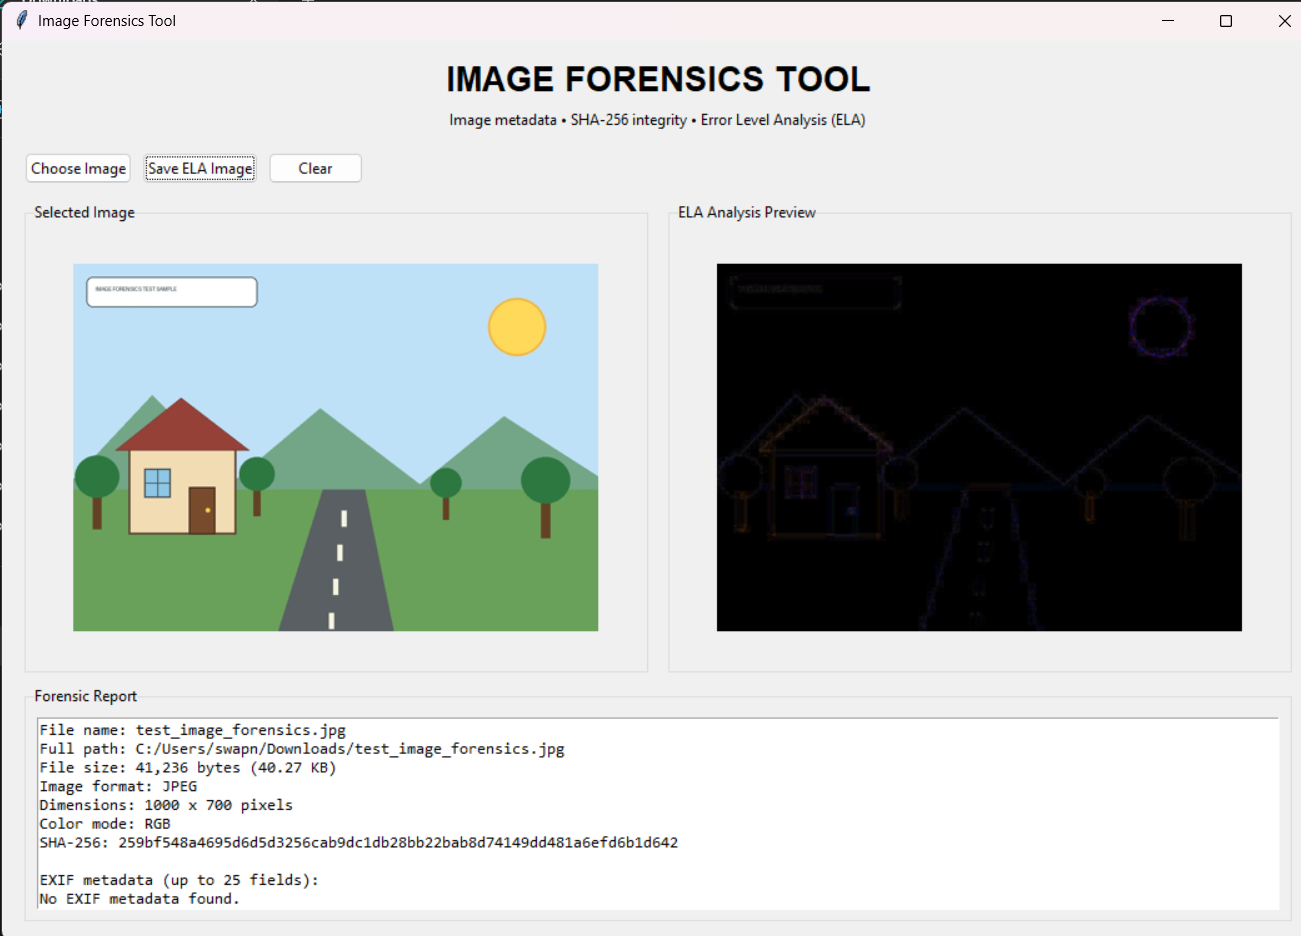
\includegraphics[width=0.85\textwidth]{1.png}
\caption{Image Forensics Tool showing the selected image and forensic report}
\end{figure}

\begin{figure}[h]
\centering
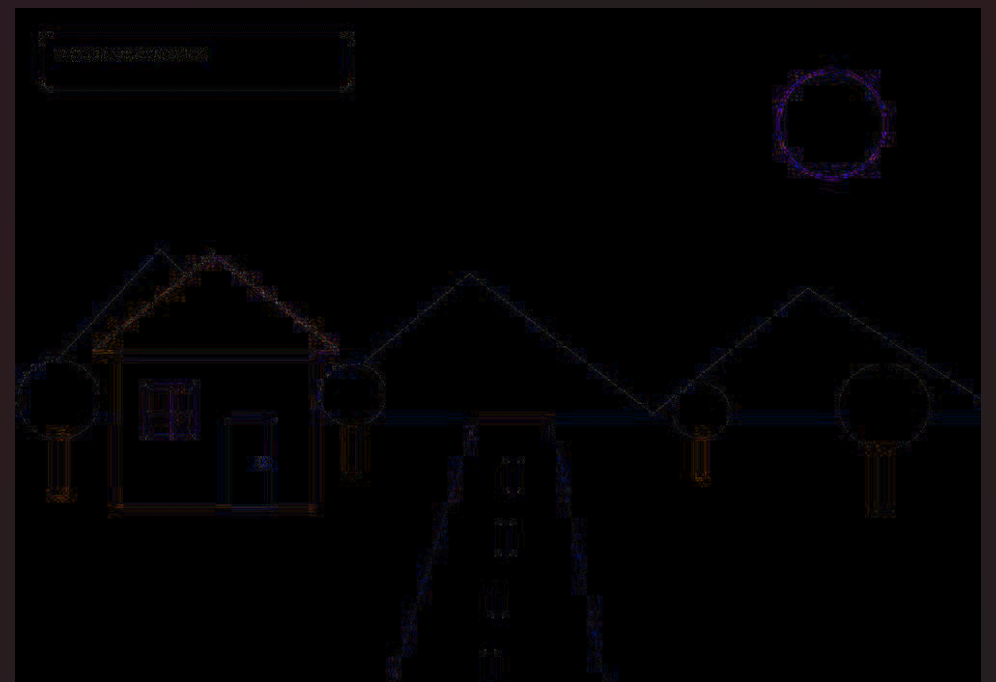
\includegraphics[width=0.7\textwidth]{2.png}
\caption{Error Level Analysis output for the sample image}
\end{figure}

\chapter{Conclusion}
The Image Forensics Tool provides a simple desktop interface for preliminary image examination. It displays image properties, available EXIF metadata, a SHA-256 hash, and an ELA preview.

\end{document}
